% @Author: AnthonyKenny98
% @Date:   2020-03-01 19:39:42
% @Last Modified by:   AnthonyKenny98
% @Last Modified time: 2020-03-01 20:52:13
    
\subsection{Instruction Set Architecture}
    An Instruction Set Architecture can be thought of as an abstract model of a computer. On a broad level, it defines the data types, memory model, and registers of a computer, along with the instructions that it can execute. \\
    It can also be thought as a ``contract'' between hardware and software developers. It is the promise made that the hardware will be able to execute all instructions defined in the \ac{ISA}, and the limitation that software must be compiled into that set of instructions.

% \begin{figure}[H]
% \begin{center}
%     \begin{subfigure}{0.4\textwidth}
%         \begin{lstlisting}[style=CStyle]
%     #include <stdio.h>
%     int main(void) {
%         c = a + b; 
%     } 
%         \end{lstlisting}
%         \caption{C Function}
%     \end{subfigure} 
%     \ \ \ \ \
%     \begin{subfigure}{0.4\textwidth}
%         \begin{lstlisting} %[style=ASM]
%     add $x3, $x1, $x2 
%         \end{lstlisting}
%         \caption{Assembly Implementation}
%     \end{subfigure}

% \caption{Example of C function and its equivalent assembly code}
% \end{center}
% \end{figure}

\subsection{RISC Processor Design}
    
    % @Author: AnthonyKenny98
% @Date:   2020-03-01 20:09:46
% @Last Modified by:   AnthonyKenny98
% @Last Modified time: 2020-04-03 13:32:58
\begin{figure}[H]
    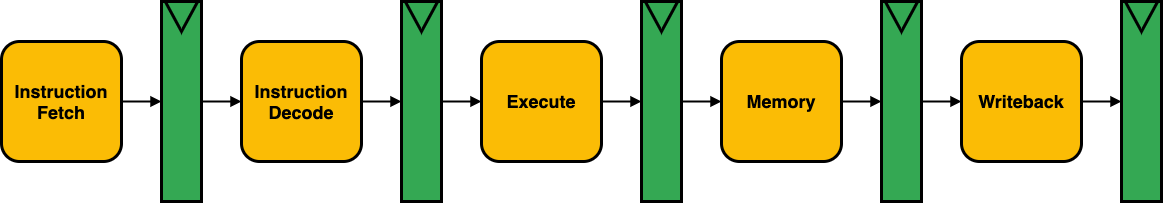
\includegraphics[draft=false,width=\linewidth]{chapters/chapter4/img/RISC-Datapath.png}
    \caption{5-Stage \gls{RISC} Datapath}
    \label{fig:RISC-Datapath}
\end{figure}